% =====================================================================================
% Paper 2: attention excitation for NVV tags (ACL format).
% Method, experiments and figures only; the introduction is a placeholder.
% Numbers: Para/eval/superbench/EXCITATION.md and out/ (judge qwen3.8-omni-flash, run1, seed 0).
% Code: nvv-tag-guidance (src/tagguide/excite.py, omnivoice.py, cosyvoice.py; bench/excite/).
% Code/method cross-check: CROSSCHECK.md in this folder.
% Build: latexmk -pdf excite.tex
% =====================================================================================
\documentclass[11pt]{article}
\usepackage[review]{acl}
\usepackage{times}
\usepackage{latexsym}
\usepackage[T1]{fontenc}
\usepackage[utf8]{inputenc}
\usepackage{microtype}
\usepackage{inconsolata}
\usepackage{graphicx}
\usepackage{booktabs}
\usepackage{amsmath,amssymb}
\usepackage{xcolor}

\newcommand{\tg}[1]{\texttt{[#1]}}
\newcommand{\todo}[1]{\textcolor{red}{[TODO: #1]}}

\title{Exciting the Tag: Attention Bias for Non-Verbal Vocalization Tags in Text-to-Speech}

\author{Anonymous}

\begin{document}
\maketitle

\begin{abstract}
\todo{abstract once the story is fixed.} Draft: TTS models given an inline tag such as \tg{laughter} often read straight through it. In a masked diffusion TTS model, the output frames where the tag's sound belongs find the tag at the first decoding step, but on the tags the model misses they stop reading it as decoding proceeds. We add a constant bias to the attention scores from those frames to the tag's text tokens, early in decoding, with no gradient and no extra forward pass. On the English tag-based part of NVV-SuperBench this raises F1 from 0.909 to 0.970 on OmniVoice and from 0.551 to 0.603 on CosyVoice~2, an autoregressive model whose window is read from its own attention, without changing intelligibility or the speaker.
\end{abstract}

\section{Introduction}
\todo{story and contributions.}

\section{Related work}
\label{sec:related}

\paragraph{Non-verbal vocalizations in TTS.} Early work synthesizes one NVV on its own, such as laughter from pseudo-phonetic tokens \citep{xin2023laughter}. Recent models instead take inline tags in the text, learned from corpora whose transcripts mark the vocalizations \citep{borisov2025nonverbaltts,liao2025nvspeech}; CosyVoice~2 \citep{du2024cosyvoice2}, Dia \citep{nari2025dia} and OmniVoice \citep{zhu2026omnivoice} are open examples. NVV-SuperBench \citep{xue2026nvvsuperbench} asks whether the tagged NVV is heard where the tag is, and finds many tags missed or misplaced. Work so far improves tags through data and training; we change only the decoding of a trained model.

\paragraph{Attention control.} In text-to-image diffusion, the cross-attention from image positions to a word decides where that word is drawn. Prompt-to-Prompt \citep{hertz2023p2p} edits an image by injecting or reweighting these maps; paint-with-words \citep{balaji2022ediffi} and DenseDiffusion \citep{kim2023dense} add a bias towards a word inside a region the user draws; Attend-and-Excite \citep{chefer2023attend} finds that a neglected subject gets too little attention in the early steps and raises it by a gradient step on the latent. In language models, PASTA \citep{zhang2024pasta} steers attention to a span the user marks by down-weighting the other tokens in selected heads. Excitation is closest to paint-with-words: a constant additive bias from known positions, with no gradient. Attend-and-Excite argues that such rescaling cannot recover a neglected subject, because an absent object has no location whose attention could be raised. A tag does have one: the window says where its sound belongs, before generation. The output is also discrete tokens, with no latent for a gradient step, and one tag of a few text tokens spans many output frames, so the bias acts from a window of frames rather than one region.

\paragraph{Two families of TTS decoders.} Codec language models such as VALL-E \citep{wang2023valle} and CosyVoice~2 emit discrete speech tokens one at a time, left to right. Masked generative models such as MaskGCT \citep{wang2025maskgct} and OmniVoice, following MaskGIT \citep{chang2022maskgit}, predict all masked tokens in parallel and commit the most confident first, over a fixed number of steps. Both commit a token once and never revise it, but in different orders, which decides when a decoding-time method can still change the output; we use one model of each family.

\paragraph{Attention as alignment in TTS.} In attention-based TTS the attention from speech to text follows the reading order; it can be pushed towards the diagonal in training \citep{tachibana2018guided}, and codec language models learn it without a duration model. We read this alignment at inference: on CosyVoice~2 it places the window, and on OmniVoice it shows where the tag is neglected.

\section{Method}
\label{sec:method}
We treat the TTS model as a transformer that decodes discrete output tokens, one per output position (and codebook), with attention from each output position to the text. At each step it predicts tokens for the open positions and commits some of them; a committed token is never revised. Section~\ref{sec:impl} gives the architecture and commit order of the two models we use.

\subsection{Attention excitation}
\label{sec:excite}
Let $T_{\text{tag}}$ be the positions of the tag's text tokens (a tag is 3--7 tokens in OmniVoice's tokenizer) and $m$ a window of output positions around the tag (Section~\ref{sec:window}). In every layer and head of the conditional pass, we add a constant $b$ to the pre-softmax attention score from each output position $i$ in the window to each tag token $j$:
\begin{equation}
\tilde s_{ij} = s_{ij} + b\,[\,i \in m \wedge j \in T_{\text{tag}}\,], \qquad s_{ij} = \frac{q_i^\top k_j}{\sqrt d}.
\label{eq:excite}
\end{equation}
If $p_i$ is the attention mass of position $i$ on the tag before the bias, after it
\begin{equation}
p_i' = \frac{p_i\, e^b}{1 - p_i + p_i\, e^b},
\label{eq:odds}
\end{equation}
so the odds of attending to the tag are multiplied by $e^b$ ($\approx 7.4$ at $b = 2$): a frame that reads the tag a little reads it much more, and one that ignores it stays near zero. We use $b = 2$. Excitation adds no forward pass and no gradient.

\subsection{Localization window}
\label{sec:window}
Let $j_s$ be the text position where the word before the tag starts, $j_e$ the one where the word after it ends, and $A(j)$ the output position at which text position $j$ is spoken. The window is
\begin{equation}
m_i = \big[\,A(j_s) - \delta \le i < A(j_e) + \delta\,\big],
\label{eq:window}
\end{equation}
where $[\cdot]$ is 1 if the condition holds and 0 otherwise, and $\delta$ is a margin for the error of $A$. The alignment $A$ is not observed. When the output length is fixed before decoding it can be estimated from durations; when it is open, the model's attention gives its inverse, the text position each output position reads (Section~\ref{sec:impl}).

\subsection{Application schedule}
\label{sec:when}
Let $a^{(t)}_{ij}$ be the attention from output position $i$ to text token $j$ at step $t$ (mean over heads and layers, without the bias), $X$ the target text's tokens, and
\begin{equation}
\alpha_t = \frac{1}{|m|} \sum_{i \in m} \frac{\sum_{j \in T_{\text{tag}}} a^{(t)}_{ij}}{\sum_{j \in X} a^{(t)}_{ij}}
\label{eq:share}
\end{equation}
the window's share of text attention on the tag. Attend-and-Excite \citep{chefer2023attend} excites only in the early denoising steps, where the image layout is decided. A tag has a similar deadline. At step 1, $\alpha_1$ is the same for the tags the model will voice and those it will miss; during decoding $\alpha_t$ falls on the missed tags, and their frames take their content from the surrounding words (Section~\ref{sec:neglect}). The bias is therefore applied with a gate $g_t \in \{0, 1\}$ that is on early:
\begin{equation}
\tilde s^{(t)}_{ij} = s^{(t)}_{ij} + b\, g_t\, \big[\,i \in m \wedge j \in T_{\text{tag}}\,\big].
\label{eq:gate}
\end{equation}
It need not stay on: after it stops, $\alpha_t$ stays above its unguided value (Figure~\ref{fig:neglect}).

\begin{figure*}[t]
  \centering
  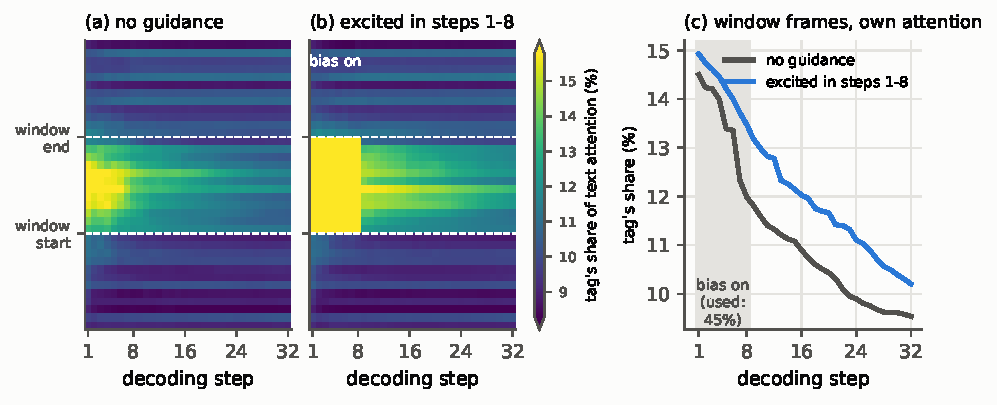
\includegraphics[width=\textwidth]{figures/fig_neglect.pdf}
  \caption{The 14 tags OmniVoice misses without guidance: how much the audio frames attend to the tag over the 32 decoding steps (mean over heads and layers; share of each frame's attention on the target text). Frames are placed relative to the tag's window (dashed lines) and averaged over the items. (a) No guidance. (b) Excitation in steps 1--8, the attention actually used (with the bias; the colour scale saturates in steps 1--8). (c) The window frames' own attention, with the bias taken out, median over the items.}
  \label{fig:neglect}
\end{figure*}

\section{Implementation}
\label{sec:impl}

\subsection{OmniVoice: masked generative decoding}
\label{sec:impl-omni}
OmniVoice \citep{zhu2026omnivoice} is a Qwen3 transformer over one sequence: a style prefix, the text (prompt transcript and target text), the voice prompt's audio tokens and the target frames, with full attention between all positions. It generates a fixed number $T$ of target frames (25 per second) by iterative unmasking: every frame starts masked, and at each of 32 steps the model predicts the masked tokens (one per frame and codebook) and commits a scheduled number of them, the most confident first, each as the arg max of its prediction. Each step decodes from classifier-free guided scores \citep{ho2022cfg} of a conditional pass and an unconditional pass on the frames alone.

\paragraph{Excitation.} The bias of Eq.~\eqref{eq:excite} is an additive attention mask on the conditional row of the batch, the same in every layer; the unconditional row does not see the text and is left unchanged.

\paragraph{Window.} The output length is fixed before decoding, so $A$ in Eq.~\eqref{eq:window} comes from the model's own duration estimator $D$:
\begin{equation}
A(j) = T\,\frac{D(x_{<j})}{D(x)},
\label{eq:align}
\end{equation}
where $x$ is the untagged text and $x_{<j}$ its first $j$ characters. $D$ is used as OmniVoice ships it: an estimate $d$ below 50 frames (2\,s) is raised to $50\,(d/50)^{1/3}$, so a boundary within the first 2\,s of speech is placed later than its share of the text (on 62 of the 150 items, by up to 20 frames). The margin is $\delta = 0.3$\,s. Over the 150 items the window is a median of 30 frames (1.2\,s; range 16--124) out of 168.

\paragraph{Schedule.} The gate is $g_t = [t \le K]$ with $K = 8$: the bias acts while the gap between voiced and missed tags is still opening, and the later steps decode unchanged. By step $t$ the schedule has committed about a share
\begin{equation}
\rho_t = \frac{\sigma\,\tau_t}{1 + (\sigma - 1)\,\tau_t}, \qquad \tau_t = t/32,\ \sigma = 0.1
\label{eq:rho}
\end{equation}
of the tokens (3\%, 9\%, 23\% and 60\% at $t = 8, 16, 24, 30$), so the whole output is still being decided while the bias acts. Section~\ref{sec:steps-res} tests later starts.

\subsection{CosyVoice~2: autoregressive decoding}
\label{sec:impl-cosy}
CosyVoice~2 \citep{du2024cosyvoice2} reads the prompt transcript and the text in a causal Qwen2 language model (LM) that emits speech tokens one at a time; a flow-matching model renders them. Each speech token is committed when it is emitted.

\paragraph{Excitation.} At a step in the window, $b$ is added to the scores from the current speech token to the tag's text tokens, in every layer and head of the LM.

\paragraph{Window.} The output length is open, so the window is read from the model. At step $t$, let $\bar a_{t,j}$ be the conditional stream's attention from the current speech token to target-text token $j$, normalized over the target text, before the bias and averaged over the heads of layers $\mathcal L = \{11, 16\}$ (0-based). The read position is
\begin{equation}
r_t = \arg\max_j\,(\kappa * \bar a_t)_j,
\label{eq:read}
\end{equation}
with $\kappa$ a three-token box filter. In these layers $r_t$ moves monotonically with $t$ (Spearman $\rho$ 0.99--1.00 on four items, against 0.08--0.45 for the mean over all layers), so it stands for $A^{-1}$, and the window of Eq.~\eqref{eq:window} becomes
\begin{equation}
m_t = \big[\,j_s - \delta \le r_{t-1} < j_e + \delta\,\big], \qquad \delta = 1\ \text{token};
\label{eq:window-cosy}
\end{equation}
the bias at step $t$ uses the read position of step $t-1$, from the current speech token. The window is on for 25--28\% of the steps.

\paragraph{Schedule.} Each speech token reads the text once, at the step that emits it, so $g_t = m_t$.

\section{Experimental setup}
\label{sec:setup}
\paragraph{Benchmark.} The English tag-based part of NVV-SuperBench \citep{xue2026nvvsuperbench}: 2,250 sentences over 45 NVV types, each with one inline marker at a word position. A model is run on the items of the types its tags cover, with the marker replaced by its own tag: for OmniVoice \tg{laughter}, \tg{sigh}, \tg{surprise-ah}, \tg{surprise-oh} and \tg{dissatisfaction-hnn} (150 items); for CosyVoice~2 breath, laughter, cough, clucking, quick breath, hissing, sigh and lip smack (400 items, 50 per type).

\paragraph{Models and voices.} Public base checkpoints without fine-tuning: OmniVoice and CosyVoice~2 0.5B. Each item is cloned from one of two fixed English voices made once with OmniVoice's voice design, with their transcripts, and synthesized once with seed 0, the same seed and voice in every setting; all OmniVoice settings, including no guidance, run through the same decoding loop. OmniVoice's upstream inference tokenizes each tag apart from the text around it, unlike its training; we tokenize the whole text at once in every setting.

\paragraph{Judge and metrics.} An audio language model hears the clip with the text and the target type and reports whether the NVV is present and before which word. This is the benchmark's verifier with Qwen3.8-Omni-Flash \citep{qwen2025omni} in place of Gemini~2.5~Pro, which no longer accepts new users; with one run, settings compare with each other but not with the published tables. A detection within 2 words of the tag is a hit, giving precision, recall and F1, and against no guidance we count the items fixed and broken (exact sign test). WER is from Whisper large-v3 \citep{radford2023whisper} against the untagged text, capped at 1 per clip (Whisper spells a long hiss as ``s-s-s\ldots''); SIM-o is the cosine similarity of WavLM-large \citep{chen2022wavlm} ECAPA-TDNN \citep{desplanques2020ecapa} embeddings of the clip and the voice prompt; both are compared per item (sign or Wilcoxon test). RTF is measured on one RTX~5070~Ti. Attention is read from the conditional pass (mean over heads and layers) on re-synthesized runs that reproduce the judged clips exactly.

\paragraph{Controls (OmniVoice).} The same bias in the same window and steps on another word's tokens (the word before the tag; the sentence's first word), and the bias in later steps (9--32, 1--32, 25--32, 29--32).

\section{Results}
\label{sec:results}

\begin{figure*}[t]
  \centering
  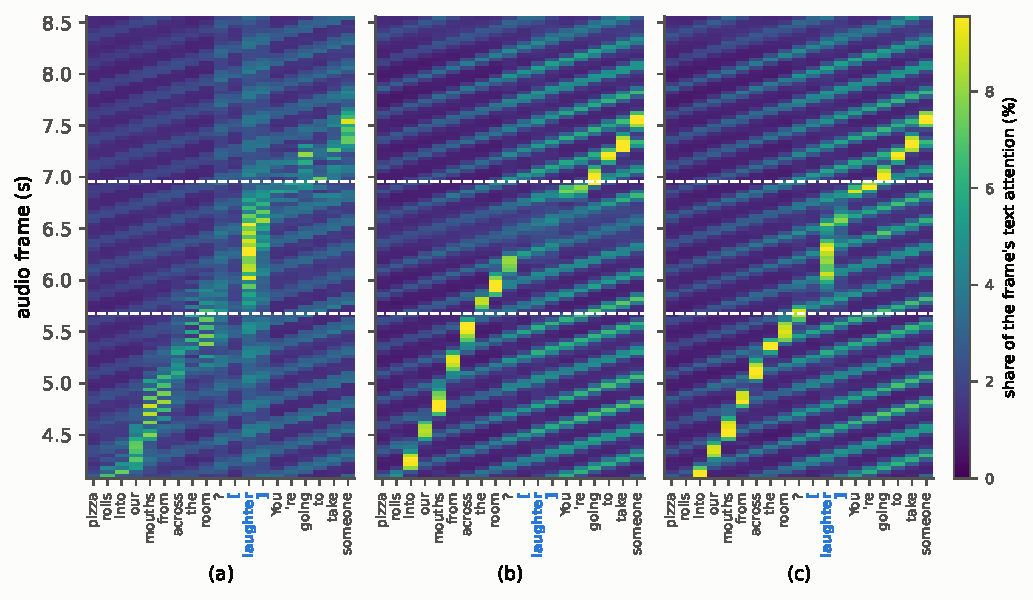
\includegraphics[width=0.8\textwidth]{figures/fig_attention.pdf}
  \caption{Where each audio frame around a missed laugh (en\_1428) reads in the text, OmniVoice. Rows: audio frames (time upward); columns: the text tokens around the tag (tag in bold blue); each row is the frame's attention on the target text (mean over heads and layers), normalized to 100\%; dashed lines: the window. Left: no guidance, step 1. Middle: no guidance, step 16. Right: excitation in steps 1--8, the model's own attention at step 16 (no bias at that step). Titles: the window frames' share of text attention on the tag.}
  \label{fig:attention}
\end{figure*}

\subsection{Main results}

\begin{table}[t]
  \centering
  \footnotesize
  \setlength{\tabcolsep}{3pt}
  \resizebox{\columnwidth}{!}{%
\begin{tabular}{llcccccc}
    \toprule
    Model & Setting & F1 & Fix/brk ($p$) & WER & SIM-o & RTF \\
    \midrule
    OmniVoice   & none       & .909 & --          & .056 & .814 & .153 \\
                & excitation & \textbf{.970} & 12/1 (.003) & .059 & .808 & .150 \\
    \midrule
    CosyVoice 2 & none       & .551 & --           & .044 & .749 & 0.80 \\
                & excitation & \textbf{.603} & 61/38 (.027) & .043 & .746 & 0.82 \\
    \bottomrule
  \end{tabular}}
  \caption{NVV-SuperBench, English tag-based part (OmniVoice 150 items, CosyVoice~2 400); one run of the substitute judge. Fix/brk: items hit with excitation and missed without, and the reverse; $p$: exact sign test. WER (capped at 1 per clip) and SIM-o: means over items.}
  \label{tab:main}
\end{table}

Excitation raises F1 from 0.909 to 0.970 on OmniVoice (12 items fixed, 1 broken, $p = .003$) and from 0.551 to 0.603 on CosyVoice~2 (61/38, $p = .027$), at the same RTF (Table~\ref{tab:main}). WER and SIM-o do not change significantly on either model (per-item sign tests, $p \ge .086$).

\subsection{Attention neglect during decoding}
\label{sec:neglect}

At step 1 the window frames attend to the tag as much for the tags the model will miss as for those it voices (AUC 0.59). During decoding this attention rises on voiced tags and falls on missed ones, which separates them by step 16 (AUC 0.73). Figure~\ref{fig:attention} shows one missed laugh: the tag's share of the window's text attention falls from 13\% at step 1 to 8\% at step 16, and the alignment runs from the word before the tag straight to the word after it. Figure~\ref{fig:neglect} shows the 14 missed tags. Without guidance the share falls from 14.5\% to 9.5\%. After excitation in steps 1--8 the model's own attention stays above the unguided run up to step 32 (1.09$\times$ over steps 9--32; higher on 13 of 14 items, $p = .002$), most in layers 8, 12 and 13 (1.42$\times$), the layers where voiced and missed tags separate during decoding (AUC 0.35 at step 1, 0.75 at step 32). Twelve of the 14 tags are then voiced.

\subsection{Effect of the bias on attention}

\begin{table}[t]
  \centering
  \footnotesize
  \resizebox{\columnwidth}{!}{%
\begin{tabular}{lccc}
    \toprule
    Attention on the tag & Natural & Excited & Ratio \\
    \midrule
    OmniVoice, window, steps 1--8 & 1.01\% & 5.08\% & $\times$5.0 \\
    CosyVoice 2, steps in window  & 0.7\%  & 2.9\%  & $\times$4.0 \\
    \bottomrule
  \end{tabular}}
  \caption{Median attention mass on the tag's tokens (mean over heads and layers) from the excited positions, without the bias (natural) and with it.}
  \label{tab:share}
\end{table}

The bias multiplies the tag's attention share by 5.0 on OmniVoice and 4.0 on CosyVoice~2 (Table~\ref{tab:share}). This is below $e^2 \approx 7.4$ because Eq.~\eqref{eq:odds} saturates in heads that already attend to the tag ($\times 4.5$ at $p_i = 0.1$) and the shares are averaged over heads. Over all 150 OmniVoice items the model's own attention after step 8 is back at the unguided level (1.12\% against 1.11\%); the lasting gain is on the missed tags.

\subsection{Placebo targets}

\begin{table}[t]
  \centering
  \small
  \setlength{\tabcolsep}{4pt}
  \begin{tabular}{lccc}
    \toprule
    Bias target & F1 & Fix/brk & Exc.\ better/worse \\
    \midrule
    the tag (excitation)   & .970 & 12/1 & -- \\
    word before the tag    & .916 & 8/8  & 13/2 (.007) \\
    sentence's first word  & .926 & 6/4  & 11/2 (.022) \\
    \bottomrule
  \end{tabular}
  \caption{Placebo, OmniVoice: the same bias in the same window and steps on another word's tokens. Fix/brk against no guidance; last column: items excitation gets right and the placebo does not, and the reverse.}
  \label{tab:placebo}
\end{table}

The same bias on another word's tokens fixes about as many items as it breaks, and excitation beats it on 13 items against 2 ($p = .007$) and 11 against 2 ($p = .022$; Table~\ref{tab:placebo}). The bias has to go to the tag.

\subsection{Start step}
\label{sec:steps-res}

\begin{table}[t]
  \centering
  \small
  \setlength{\tabcolsep}{4pt}
  \begin{tabular}{lcccc}
    \toprule
    Steps & Committed & F1 & Fix/brk & vs 1--8 \\
    \midrule
    1--8   & 0\%  & .970 & 12/1 & -- \\
    9--32  & 3\%  & .973 & 10/0 & 3/2 (1) \\
    1--32  & 0\%  & .970 & 13/2 & 1/1 \\
    25--32 & 23\% & .933 & 5/1  & 8/1 (.039) \\
    29--32 & 41\% & .919 & 3/3  & 12/1 (.003) \\
    \bottomrule
  \end{tabular}
  \caption{Excitation in later steps, OmniVoice. Committed: share of the target's tokens committed when the bias starts. Last column: items the 1--8 setting gets right and this one does not, and the reverse.}
  \label{tab:steps}
\end{table}

Starting the bias at step 9, while the gap between voiced and missed tags is still opening, keeps the gain. Starting at step 25 or 29, after the gap has settled (mean AUC 0.75 from step 20), loses most or all of it (Table~\ref{tab:steps}). The 9--32 setting also excites for 24 steps instead of 8, so the table shows when the bias must start, not how long it must last.

\section*{Limitations}
One seed, one run of a substitute judge, and few missed items on OmniVoice (14 of 150), so differences of a few items are trends. The attention analysis of Section~\ref{sec:neglect} is on OmniVoice only. The CosyVoice~2 window depends on two LM layers chosen on four items. No listening test.

\bibliography{refs}

\end{document}
